\section{Auswertung}
\label{sec:Auswertung}
\FloatBarrier
\subsection{Bestimmung des Emissionsspektrums}
Zunächst wurde das Emissionsspektrum der Röntgenröhre gemessen, die dabei aufgenommenen Wert sind in Tabelle \ref{tab:emission1} und \ref{tab:emmision2} zu finden.
\begin{table}
\centering
  \caption{Die aufgenommen Intensitäten der Röntgenröhre nach Reflexion an einem LiF-Kristall [Teil 1].}
  \begin{tabular}[t]{cc}
  \toprule
  $\alpha \,/\, \si{\degree} $ & $\frac{N}{Imp/\si{\second}}$\\
  \midrule
  8.0 & 323.0 \\
  8.1 & 316.0\\
  8.2 & 326.0\\
  8.3 & 340.0\\
  8.4 & 335.0\\
  8.5 & 343.0\\
  8.6 & 350.0\\
  8.7 & 350.0\\
  8.8 & 366.0\\
  8.9 & 357.0\\
  9.0 & 371.0\\
  9.1 & 371.0\\
  9.2 & 372.0\\
  9.3 & 364.0\\
  9.4 & 381.0\\
  9.5 & 379.0\\
  9.6 & 393.0\\
  9.7 & 375.0\\
  9.8 & 391.0\\
  9.9 & 395.0\\
  10.0 & 402.0\\
  10.1 & 405.0\\
  10.2 & 390.0\\
  10.3 & 398.0\\
  10.4 & 400.0\\
  10.5 & 418.0\\
  10.6 & 401.0\\
  10.7 & 410.0\\
  10.8 & 408.0\\
  \bottomrule
  \end{tabular}
  \begin{tabular}[t]{cc}
  \toprule
  $\alpha \,/\, \si{\degree} $ & $\frac{N}{Imp/\si{\second}}$ \\
  \midrule
  10.9 & 409.0\\
  11.0 & 414.0\\
  11.1 & 420.0\\
  11.2 & 417.0\\
  11.3 & 417.0\\
  11.4 & 409.0\\
  11.5 & 406.0\\
  11.6 & 404.0\\
  11.7 & 405.0\\
  11.8 & 400.0\\
  11.9 & 383.0\\
  12.0 & 389.0\\
  12.1 & 382.0\\
  12.2 & 372.0\\
  12.3 & 376.0\\
  12.4 & 385.0\\
  12.5 & 384.0\\
  12.6 & 382.0\\
  12.7 & 373.0\\
  12.8 & 376.0\\
  12.9 & 373.0\\
  13.0 & 375.0\\
  13.1 & 366.0\\
  13.2 & 354.0\\
  13.3 & 341.0\\
  13.4 & 326.0\\
  13.5 & 318.0\\
  13.6 & 305.0\\
  13.7 & 296.0  \\
  \bottomrule
  \end{tabular}
  \begin{tabular}[t]{cc}
  \toprule
  $\alpha \,/\, \si{\degree} $ & $\frac{N}{Imp/\si{\second}}$ \\
  \midrule
  13.8 & 286.0  \\
  13.9 & 285.0  \\
  14.0 & 274.0  \\
  14.1 & 264.0  \\
  14.2 & 266.0  \\
  14.3 & 270.0  \\
  14.4 & 255.0  \\
  14.5 & 255.0  \\
  14.6 & 260.0  \\
  14.7 & 251.0  \\
  14.8 & 250.0  \\
  14.9 & 248.0  \\
  15.0 & 253.0  \\
  15.1 & 257.0  \\
  15.2 & 248.0  \\
  15.3 & 242.0  \\
  15.4 & 249.0  \\
  15.5 & 246.0  \\
  15.6 & 252.0  \\
  15.7 & 236.0  \\
  15.8 & 234.0  \\
  15.9 & 231.0  \\
  16.0 & 215.0  \\
  16.1 & 217.0  \\
  16.2 & 227.0  \\
  16.3 & 214.0  \\
  16.4 & 217.0  \\
  16.5 & 210.0  \\
  \bottomrule
  \end{tabular}
  \label{tab:emission1}
\end{table}

\begin{table}
  \centering
  \caption{Die aufgenommen Intensitäten der Röntgenröhre nach Reflexion an einem LiF-Kristall [Teil 2].}
  \begin{tabular}[t]{cc}
  \toprule
  $\alpha \,/\, \si{\degree} $ & $\frac{N}{Imp/\si{\second}}$ \\
  \midrule
  16.6 & 211.0  \\
  16.7 & 206.0  \\
  16.8 & 205.0  \\
  16.9 & 198.0  \\
  17.0 & 203.0  \\
  17.1 & 199.0  \\
  17.2 & 198.0  \\
  17.3 & 191.0  \\
  17.4 & 192.0  \\
  17.5 & 184.0  \\
  17.6 & 191.0  \\
  17.7 & 188.0  \\
  17.8 & 181.0  \\
  17.9 & 185.0  \\
  18.0 & 184.0  \\
  18.1 & 179.0  \\
  18.2 & 180.0  \\
  18.3 & 166.0  \\
  18.4 & 173.0  \\
  18.5 & 167.0  \\
  18.6 & 169.0  \\
  18.7 & 160.0  \\
  18.8 & 159.0  \\
  18.9 & 157.0  \\
  19.0 & 149.0  \\
  19.1 & 153.0  \\
  19.2 & 150.0  \\
  19.3 & 147.0  \\
  19.4 & 150.0\\
  \bottomrule
  \end{tabular}
  \begin{tabular}[t]{cc}
  \toprule
  $\alpha \,/\, \si{\degree} $ & $\frac{N}{Imp/\si{\second}}$ \\
  \midrule
  19.5 & 148.0\\
  19.6 & 149.0\\
  19.7 & 143.0\\
  19.8 & 153.0\\
  19.9 & 182.0\\
  20.0 & 291.0\\
  20.1 & 1127.0\\
  20.2 & 1599.0\\
  20.3 & 1533.0\\
  20.4 & 1430.0\\
  20.5 & 1267.0\\
  20.6 & 425.0\\
  20.7 & 241.0\\
  20.8 & 225.0\\
  20.9 & 192.0\\
  21.0 & 188.0\\
  21.1 & 172.0\\
  21.2 & 168.0\\
  21.3 & 169.0\\
  21.4 & 166.0\\
  21.5 & 170.0\\
  21.6 & 174.0\\
  21.7 & 164.0\\
  21.8 & 180.0\\
  21.9 & 179.0\\
  22.0 & 191.0\\
  22.1 & 232.0\\
  22.2 & 300.0\\
  22.3 & 536.0\\
  \bottomrule
  \end{tabular}
  \begin{tabular}[t]{cc}
  \toprule
  $\alpha \,/\, \si{\degree} $ & $\frac{N}{Imp/\si{\second}}$ \\
  \midrule
  22.4 & 4128.0\\
  22.5 & 5050.0\\
  22.6 & 4750.0\\
  22.7 & 4571.0\\
  22.8 & 4097.0\\
  22.9 & 901.0\\
  23.0 & 244.0\\
  23.1 & 179.0\\
  23.2 & 151.0\\
  23.3 & 145.0\\
  23.4 & 130.0\\
  23.5 & 121.0\\
  23.6 & 126.0\\
  23.7 & 117.0\\
  23.8 & 112.0\\
  23.9 & 110.0\\
  24.0 & 105.0\\
  24.1 & 106.0\\
  24.2 & 107.0\\
  24.3 & 95.0\\
  24.4 & 94.0\\
  24.5 & 100.0\\
  24.6 & 91.0\\
  24.7 & 85.0\\
  24.8 & 88.0\\
  24.9 & 83.0\\
  25.0 & 85.0\\
  \bottomrule
  \end{tabular}
  \label{tab:emmision2}
\end{table}
\FloatBarrier

Um die charakteristischen Linien des Spektrums besser erkennen zu können wurden die Werte in der Abbildung \ref{fig:emission} aufgetragen.
Zur Erstellung des Plots und aller weiteren Plots wurde das Python Plugin matplotlib \cite{matplotlib} genutzt.
\begin{figure}
  \centering
  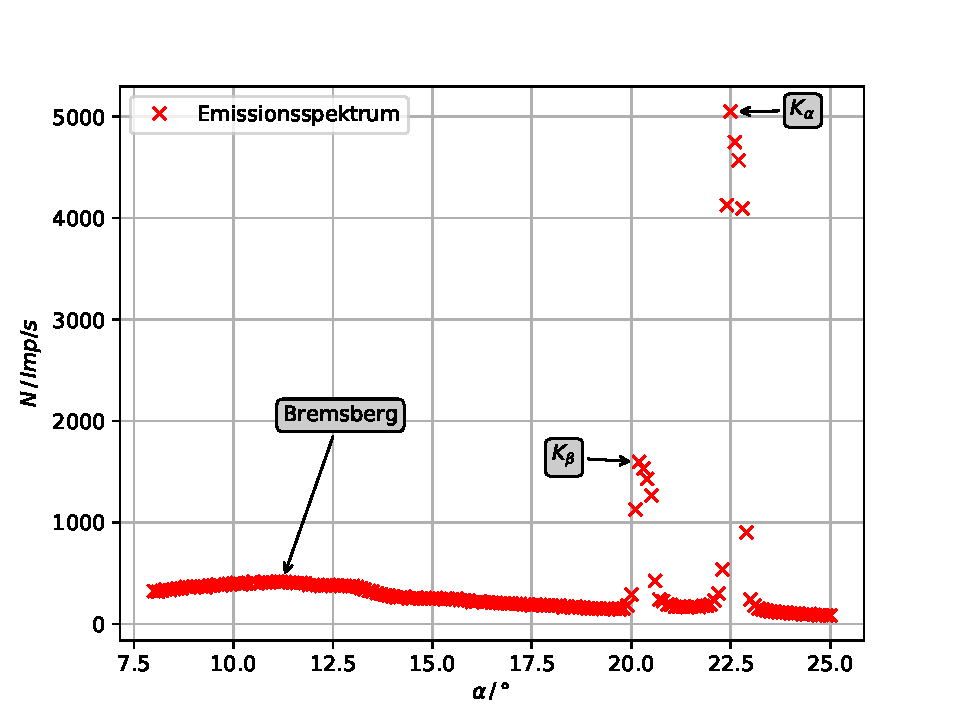
\includegraphics[width=\textwidth]{content/data/Emission.pdf}
  \caption{Die gemessen Impulse in Abhängigkeit vom Winkel $\alpha$, zusätzlich wurden Bremsberg, $K_\alpha$ und $K_\beta$ markiert.}
  \label{fig:emission}
\end{figure}

Aus der Graphik \ref{fig:emission} ist zu entnehmen, dass die gemessenen Impulse pro Sekunde bei dem Winkel $\alpha_1 = 20.2 \si{\degree}$, sowie dem Winkel $\alpha_2 = 22.5 \si{\degree}$ stark zunehmen.
Diese beiden Punkte sind in der Graphik mit $K_\beta$ für den Winkel $\alpha_1$ und $K_\alpha$ für den Winkel $\alpha_2$ gekennzeichnet worden.
Mit Hilfe der Gleichung \eqref{eq:bragg} lässt für die beiden Winkeln die Wellenlänge der reflektierten Strahlung berechnen.
Mit dieser kann nun die Energie der Strahlung berechnet werden.
Dazu wird die Gleichung
\begin{equation}
  E = \frac{ch}{\lambda}
  \label{eq:energie}
\end{equation}
genutzt.
$c$ ist hier die Lichtgeschwindigkeit und $h$ die Plank'sche Konstante.
Durch die Rechnung kann die Energie der $K_\beta$ und $K_\alpha$ Linie bestimmt werden.
\begin{align*}
  E(K_\beta) & = \SI{1.4282e-15}{\joule}\\
  E(K_\alpha) &= \SI{1.2886e-15}{\joule}\\
\end{align*}
Die hier angegebenen Unsicherheiten wurden mit dem Python Plugin uncertainties \cite{uncertainties} berechnet.
Dieses nutzt zur Berechnung der Fehler die Gauß'sche Fehlerfortpflanzungs Formel
\begin{equation*}
  \Delta y = \frac{\delta y}{\delta x_1} \cdot \Delta x_1 + ....
\end{equation*}

%Ab hier nummer 2 also T(lambda) und so  

\FloatBarrier

\subsection{Bestimmung der Transmissionsfunktion}
Die Werte in Tabelle \ref{tab:comp} ergeben sich, wie im Abschnitt \ref{sec:Durchführung} beschrieben, wenn der Kristall auf $7\si{\degree}$ eingestellt wird und schrittweise nach jeder Messung bis auf $10\si{\degree}$ erhöht wird.
Dabei sind die Messwerte der Messung ohne Absorber in der mittleren Spalte $N_0$ und die mit Absorber in der rechten Spalte $N_\text{Al}$ zu finden.
Die Messwerte können anschließen mit der Gleichung \eqref{eq:intens} in eine Intensität umgerechnet werden.
Aus dem Verhältnis der Intensität
\begin{align*} 
T(\lambda) = \frac{I_\text{Al}}{I_0},
\end{align*}
also der Intensität mit Absorber geteilt durch die des ohne Absorbers, lässt sich nun eine Transmission $T(\lambda)$ berechnen.
Diese ist abhängig von der Wellenlänge $\lambda$ und wird in Abbildung \ref{fig:trans} gegen diese aufgetragen.
Die Regressionsgerade wurde nach dem Muster $f(x) = ax+b$ erstellt.
Dabei ergibt sich für die Steigung $a$ und für den Startwert $b$ die Werte
\begin{align*}
  a & =  \SI{-0.01461(25)}{\frac{1}{\pico\meter}} \\
  b & =   \SI{1.189(16)}{} \\
\end{align*}
Zur Berechnung der Regressionsgerade wurde das Python Plugin scipy \cite{scipy} genutzt.
\begin{table}
  \centering
  \caption{Die aufgenommenen Messwerte, bei Messung mit Absorber und ohne Absorber.}
  \begin{tabular}[t]{ccc}
  \toprule
  $\alpha \,/\, \si{\degree}$ & $\frac{N_0}{Imp/\si{\second}}$ & $\frac{N_\text{Al}}{Imp/\si{\second}}$ \\
  \midrule
  7.0 & 226.0 & 113.5 \\
  7.1 & 232.0 & 112.0\\
  7.2 & 240.5 & 112.0\\
  7.3 & 248.0 & 113.5\\
  7.4 & 255.0 & 115.0\\
  7.5 & 262.0 & 113.5\\
  7.6 & 269.0 & 113.0\\
  7.7 & 276.0 & 114.5\\
  7.8 & 281.0 & 114.0\\
  7.9 & 289.5 & 112.0\\
  8.0 & 295.0 & 109.5\\
  8.1 & 300.0 & 109.0\\
  8.2 & 308.5 & 108.0\\
  8.3 & 311.0 & 106.0\\
  8.4 & 317.0 & 104.5\\
  \bottomrule
\end{tabular}
\begin{tabular}[t]{ccc}
  \toprule
  $\alpha \,/\, \si{\degree}$ & $\frac{N_0}{Imp/\si{\second}}$ & $\frac{N_\text{Al}}{Imp/\si{\second}}$ \\
  \midrule
  8.5 & 324.0 & 101.5\\
  8.6 & 328.5 & 100.0\\
  8.7 & 332.5 & 100.5\\
  8.8 & 337.0 & 97.5\\
  8.9 & 340.5 & 95.0\\
  9.0 & 348.0 & 92.5\\
  9.1 & 350.0 & 89.5\\
  9.2 & 353.0 & 88.0\\
  9.3 & 356.5 & 84.5\\
  9.4 & 359.0 & 83.0\\
  9.5 & 363.5 & 81.0\\
  9.6 & 367.0 & 78.5\\
  9.7 & 369.0 & 76.0\\
  9.8 & 370.5 & 74.0\\
  9.9 & 375.0 & 72.0\\
  10.0 & 375.5 & 68.5\\
  \bottomrule
  \end{tabular}
  \label{tab:comp}
\end{table}


\begin{figure}
  \centering
  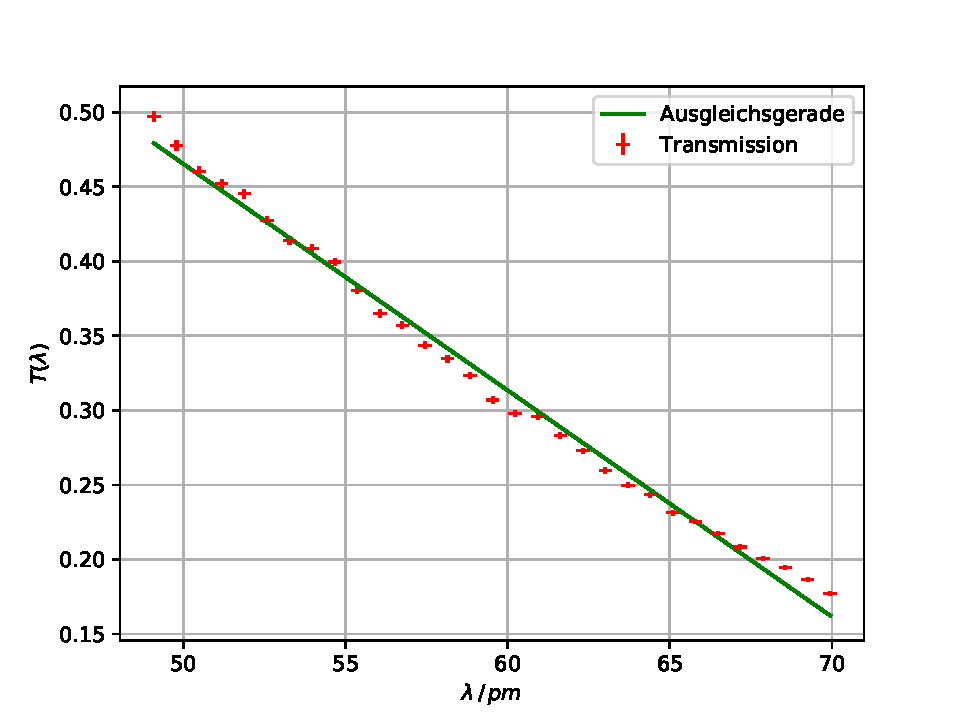
\includegraphics[width=\textwidth]{content/data/Transmission.pdf}
  \caption{Die Transmission in abhängig von $\lambda$, außerdem wurde eine Regressionsgerade erstellt.}
  \label{fig:trans}
\end{figure}

\FloatBarrier
\subsection{Berechnung der Comptonwellenlänge}
Um nun die Comptonwellenlänge zu berechnen, wurde wie im letzten Teil des Abschnitts \ref{sec:Durchführung} beschrieben, die Intensität der Strahlung drei weitere Male gemessen.
Ein Mal ohne jegliche Absorber, im folgenden ist diese $I_0$, ein weiteres Mal mit Absorber zwischen Röhre und Streuer, diese wird $I_1$ genannt und mit einem Absorber zwischen Streuer und Zählrohr hier $I_2$.
Die Comptonwellenlänge ergibt sich wie in \ref{sec:Theorie} beschrieben aus der Differenz zwischen $\lambda_2$ und $\lambda_1$.
Um die Wellenlängen zu erhalten stellen wir die Funktion der Ausgleichgerade nach $\lambda$ um.
Nun berechnen wir aus den Intensität die verschiedenen Transmissionswerte $T_1$ und $T_2$ für die unbekannten Wellenlängen $\lambda_1$ und $\lambda_2$.
Diese ergeben sich, wie oben bereits beschrieben aus dem Verhältnis $T = \frac{I_0}{I_\text{N}}$.
So erhalten wir
\begin{align*}
  T_1 & = 0.432 \\
  T_2 & = 0.374 \\
\end{align*}
Diese Werte setzten wir in die umgestellte Ausgleichsgerade ein und erhalten die Werte
\begin{align*}
  \lambda_1 &= \SI{51.8(14)}{\pico\meter}\\
  \lambda_2 &= \SI{55.7(14)}{\pico\meter}\\
\end{align*}
Aus der Differenz der beiden Werte ergibt sich schließlich die Comptonwellenlänge
\begin{align*}
  \lambda_\text{C} &= \SI{3.91(7)}{\pico\meter}
\end{align*}